\section{Gems}
\frame{
	\begin{block}{}
  	\begin{center}
  	\huge{System - Gems}
	\end{center}
  	\end{block}
}			

\subsection{API - REST in System}
\frame{
	\frametitle{API - REST in System}
	\begin{block}{URL}
		\url{http://www.example.com/?page=start}
	\end{block}
	\begin{block}{Regeln}
		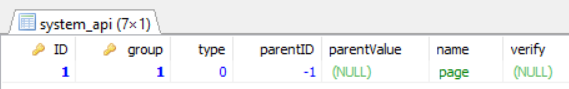
\includegraphics[width=9cm]{img/sql_system_api.png}
	\end{block}
	\begin{block}{Funktion}
		public static function page\_start()
	\end{block}	
}
\frame[t]{
	\frametitle{API Class Beispiel}
	\begin{backgroundblock}{1cm}{2.5cm}
		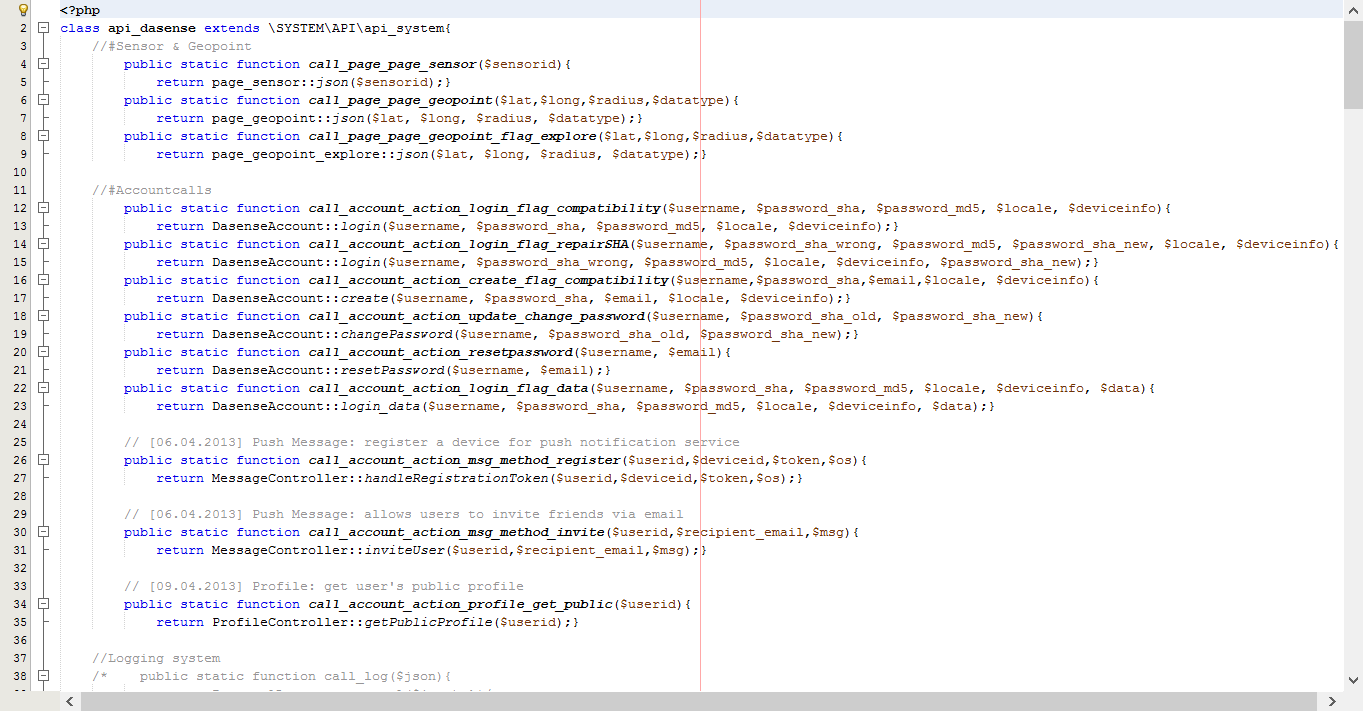
\includegraphics[width=10cm]{img/api_dasense.png}
	\end{backgroundblock}
}

\subsection{Quick Query - Sichere SQL Querys}
\frame{
	\frametitle{Quick Query - Sichere SQL Querys}
	\begin{block}{QQ}
		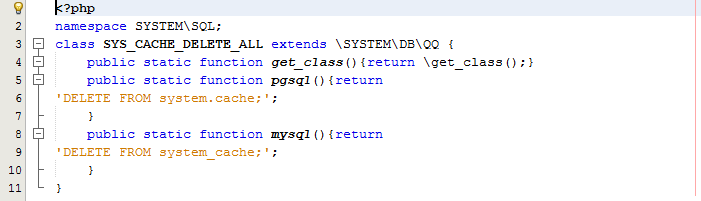
\includegraphics[width=8cm]{img/qq.png}
	\end{block}
	\begin{block}{QP}
		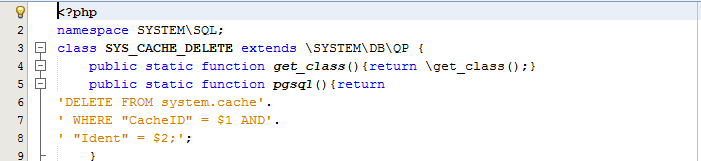
\includegraphics[width=8cm]{img/qp.png}
	\end{block}
}

\frame{
	\frametitle{Quick Query - Sichere SQL Querys}
	\begin{block}{Q1 - Eine Zeile}
		\$res = SYS\_SAIMOD\_API\_SELECT::Q1(array(\$ID,\$group));
	\end{block}
	\begin{block}{QA - Alle Zeilen}
		\$res = SYS\_SAIMOD\_API\_SELECT::QA(array(\$ID,\$group));
	\end{block}
	\begin{block}{QQ - Selber Interrieren}
		\$res = SYS\_SAIMOD\_API\_SELECT::QQ(array(\$ID,\$group));
	\end{block}
	\begin{block}{QI - Einfügen/Löschen}
		\$res = SYS\_SAIMOD\_API\_SELECT::QI(array(\$ID,\$group));
	\end{block}
}